\documentclass[a4paper]{article}


\usepackage[T1]{fontenc}    
\usepackage[utf8]{inputenc} 
\usepackage{textcomp}      
\date{} 					
\author{}                   
\usepackage{geometry}		
\geometry{ left=2cm, right=2cm, top=2cm, bottom=4cm, bindingoffset=5mm}

\usepackage{listings}
\usepackage{color}
\usepackage{longtable}

\definecolor{mygreen}{rgb}{0,0.6,0}
\definecolor{mygray}{rgb}{0.5,0.5,0.5}
\definecolor{mymauve}{rgb}{0.58,0,0.82}
\definecolor{eminence}{RGB}{108,48,130}
\definecolor{myblue}{RGB}{65,105,225}


\lstset{
	keywordstyle=\color{myblue},  
	numbers=left,  
	stringstyle=\color{mymauve},
	numberstyle=\tiny\color{mygray} ,    
	commentstyle=\fontsize{9}{13}\itshape\color{mygreen}
}

\lstset{literate=
	{á}{{\'a}}1 {é}{{\'e}}1 {í}{{\'i}}1 {ó}{{\'o}}1 {ú}{{\'u}}1
	{Á}{{\'A}}1 {É}{{\'E}}1 {Í}{{\'I}}1 {Ó}{{\'O}}1 {Ú}{{\'U}}1
	{à}{{\`a}}1 {è}{{\`e}}1 {ì}{{\`i}}1 {ò}{{\`o}}1 {ù}{{\`u}}1
	{À}{{\`A}}1 {È}{{\'E}}1 {Ì}{{\`I}}1 {Ò}{{\`O}}1 {Ù}{{\`U}}1
	{ä}{{\"a}}1 {ë}{{\"e}}1 {ï}{{\"i}}1 {ö}{{\"o}}1 {ü}{{\"u}}1
	{Ä}{{\"A}}1 {Ë}{{\"E}}1 {Ï}{{\"I}}1 {Ö}{{\"O}}1 {Ü}{{\"U}}1
	{â}{{\^a}}1 {ê}{{\^e}}1 {î}{{\^i}}1 {ô}{{\^o}}1 {û}{{\^u}}1
	{Â}{{\^A}}1 {Ê}{{\^E}}1 {Î}{{\^I}}1 {Ô}{{\^O}}1 {Û}{{\^U}}1
	{œ}{{\oe}}1 {Œ}{{\OE}}1 {æ}{{\ae}}1 {Æ}{{\AE}}1 %{ß}{{\ss}}1
	{ű}{{\H{u}}}1 {Ű}{{\H{U}}}1 {ő}{{\H{o}}}1 {Ő}{{\H{O}}}1
	{ç}{{\c c}}1 {Ç}{{\c C}}1 {ø}{{\o}}1 {å}{{\r a}}1 {Å}{{\r A}}1
}


\usepackage{graphicx}
\usepackage{xcolor}
\usepackage{hyperref} 
\usepackage{fancyhdr}
\usepackage{amsmath}											
\pagestyle{fancy}
\fancyhf{}
\fancyhead[R]{2973140 - Felix Bühler  \\ 2893121 - Jan Leusmann \\  3141241 - Jamie Ullerich}
\fancyhead[L]{Scientific Visualisation \\ Sommersemester 2019 }
\renewcommand{\headrulewidth}{0.5pt} 				

\title{Exercise 8}

\begin{document}

\maketitle 
\thispagestyle{fancy}


\section*{Exercise 8.1 - Asymptotic Decider}

Midpoint:

\begin{align*}
	c &= \dfrac{1}{4}*(f_{i,j} + f_{i+1,j} + f_{i,j+1} + f_{i+1,j+1})\\
	&= \dfrac{1}{4}*(-40 + 8 + 80 -40)\\
	&= 2
\end{align*}

Because $ c > 0 $, our lines are drawn the following:\\
Our top root is connected to our left root, and our bottom root is connected to our right root. We now
just need to calculate our asymptotes:

\begin{align*}
x_c &= \dfrac{f(0)}{f(1) - f(0)}\\
x_c(SouthWest, SouthEast) &= \dfrac{5}{6}\\
x_c(NorthWest, NorthEast) &= \dfrac{2}{3}\\
x_c(NorthEast, SouthEast) &= \dfrac{1}{6}\\
x_c(NorthWest, SouthWest) &= \dfrac{1}{3}
\end{align*}

\section*{Exercise 8.2 - Octrees}

32bit floating point $\rightarrow$ 4bytes for each voxel\\
only the last layer needs to store these voxels wich contains $ 500*500*200 = 50.000.000 $ nodes
\begin{align*}
8^x \leq 50.000.000 \Rightarrow x &= 9\\
layer_{9} &= 8^9 = 134.217.728 \text{ leaves}\\
layer_{8} &= 8^8 = 16.777.216 \text{ leaves}\\
layer_{7} &= 8^7 = 2.097.152 \text{ leaves}\\
layer_{6} &= 8^6 = 262.144 \text{ leaves}\\
layer_{5} &= 8^5 = 32.768 \text{ leaves}\\
layer_{4} &= 8^4 = 4096 \text{ leaves}\\
layer_{3} &= 8^3 = 512 \text{ leaves}\\
layer_{2} &= 8^2 = 64 \text{ leaves}\\
layer_{1} &= 8^1 = 8 \text{ leaves}\\
layer_{0} &= 8^0 = 1 \text{ leaves}
\end{align*}

\subsection*{(a)}
\begin{align*}
&= 134.217.728 * 4 \text{ bytes}\\
&= 536870912\\
&\approx 537\text{ MB}
\end{align*}
\subsection*{(b)}
\begin{align*}
&= 134.217.728 + 2*(16.777.216 + 2.097.152 + 262.144 + 32.768 + 4096 + 512 + 64 + 8 + 1)\\
&= 172.565.650 * 4 \text{ bytes} \\
&= 690262600 \text{ bytes}\\
&\approx 690 \text{MB}
\end{align*}

\newpage
\section*{Exercise 8.3 - Color Mapping with Shaders}

\begin{figure}[!ht]
	\centering
	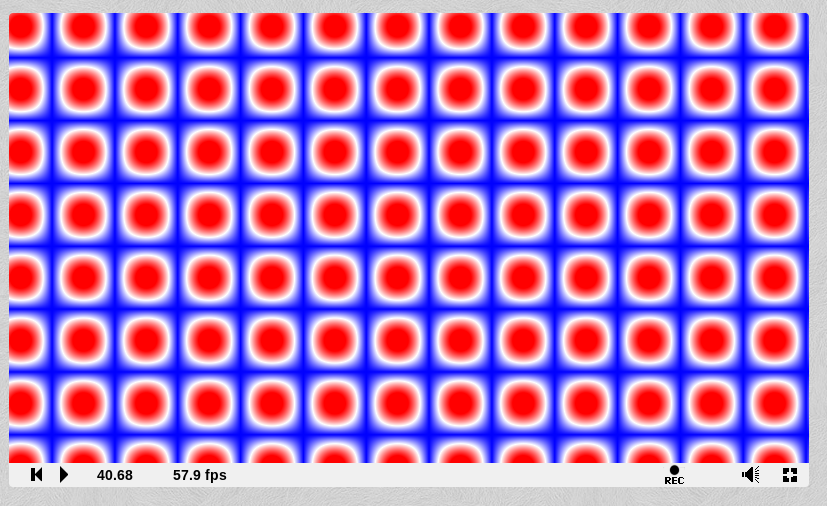
\includegraphics[width=0.7\linewidth]{Screenshot-2019-06-04_142043}
	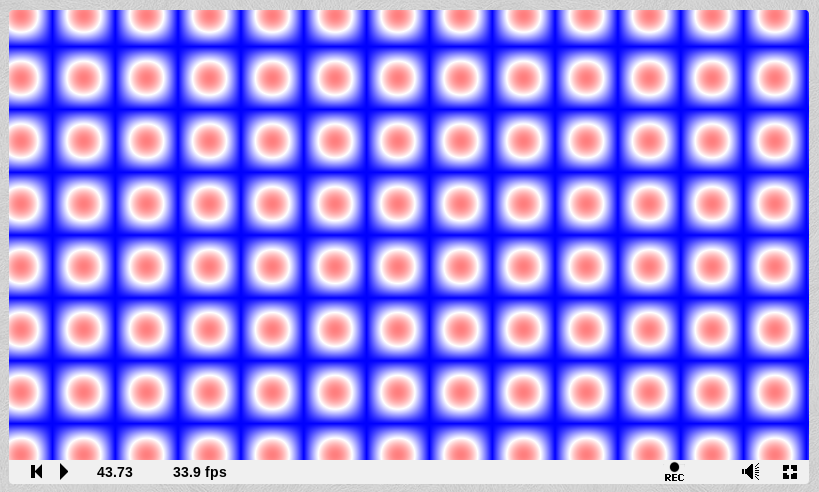
\includegraphics[width=0.7\linewidth]{Screenshot-2019-06-04_142159}
	\caption{Screenshots}
	\label{fig:screenshot-2019-06-04142043}
\end{figure}




\end{document}